\documentclass[10pt]{article}
\usepackage{fancyhdr}
\usepackage{hyperref}
\usepackage{dirtree}
\usepackage[margin=0.6in]{geometry}
\usepackage{graphicx}

\title{Mini Game Hub\\ CS-108 Project}
\author{Yogi \& Praneeth}
\date{April 2026}

\pagestyle{fancy}
\lhead{Mini Game Hub}
\rhead{Yogi \& Praneeth}

\begin{document}

    \maketitle
    \begin{abstract}
    This report is about the development of the Mini Game Hub, a secure, multi-user platform that combines Bash scripting for user authentication and Python (Pygame) for gameplay. Two authenticated players can select a game from the menu, play through a graphical interface, and save their results to a persistent leaderboard. 
    \end{abstract}

    \tableofcontents
    \newpage

    \section{Introduction}
    The Mini Game Hub is a pygame,bash platform where two players can log in and compete in various board games. The system's architecture focuses on two main areas: security (using SHA-256 hashing for passwords) and efficient game logic using NumPy matrix operations.

    \section{Libraries and Tools}
    \begin{itemize}
        \item \textbf{Bash / Shell:} Used for the authentication of the system and formatting the terminal-based leaderboard.
        \item \textbf{Pygame-CE:} Used to build the GUI and handle real-time user input.
        \item \textbf{NumPy:} Used for board representations and win-condition slicing to keep the game logic fast and efficient.
        \item \textbf{Matplotlib:} Used to generate post-game analytics, including bar and pie charts.
    \end{itemize}

    \section{System Architecture}
    \subsection{Directory Structure}
    \dirtree{%
        .1 cs108-project/.
        .2 main.sh \dots{} (Entry point \& Auth).
        .2 game.py \dots{} (Main Menu \& Selection).
        .2 leaderboard.sh \dots{} (Bash Statistics).
        .2 matplot.py \dots{} (Analytics).
        .2 users.tsv \dots{} (Hashed Credentials).
        .2 history.csv \dots{} (Game Records).
        .2 games/.
        .3 base\_game.py \dots{} (Parent Class).
        .3 tictactoe.py.
        .3 othello.py.
        .3 connect4.py.
        .2 report.tex.
        .2 Makefile.
    }

    \section{Features}
    \begin{itemize}
        \item \textbf{User Authentication:} A secure login system using SHA-256 hashing to protect the user passwords.
        \item \textbf{Multi-Game Support:} Includes full versions of Tic-Tac-Toe, Othello, and Connect 4.
        \item \textbf{Turn-Based Game play:} A reliable system for managing player turns and game flow.
        \item \textbf{Win Detection:} Optimized algorithms that instantly detect winning conditions.
        \item \textbf{Leaderboard System:} Tracks player wins and losses over time.
        \item \textbf{Data Persistence:} All match records are saved in CSV format.
        \item \textbf{Data Visualization:} Automatically generates and opens the performance graphs using Matplotlib.
        \item \textbf{Menu Interface:} A user-friendly GUI for easy navigation and game selection.
    \end{itemize}
    \newpage
      \begin{figure}[h]
    \centering
    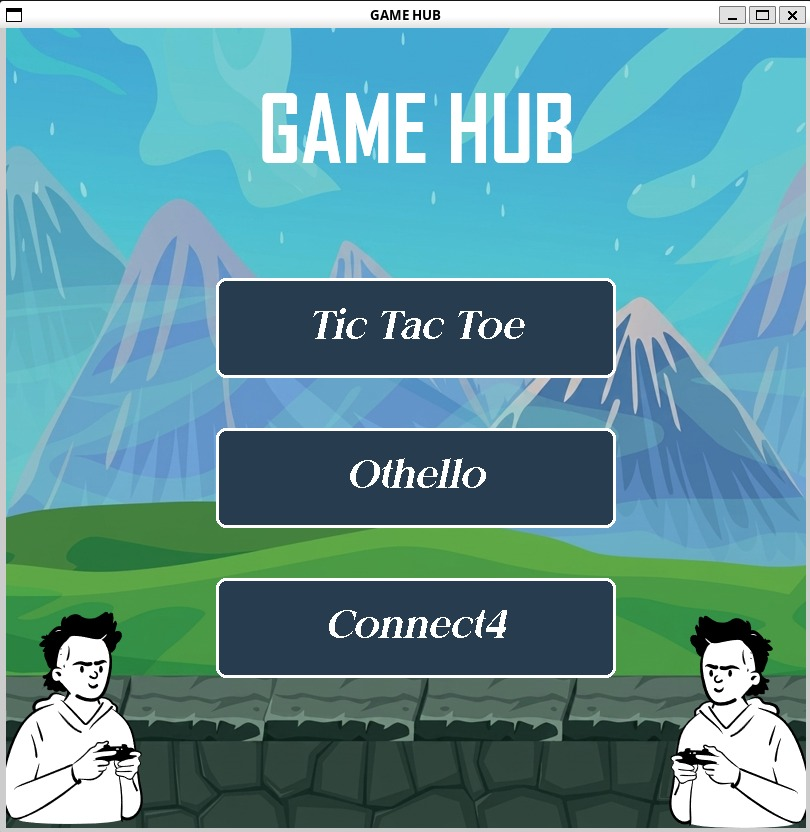
\includegraphics[width=0.5\textwidth]{gamehub.png}
    \caption{The Mini Game Hub Main Menu Interface}
    \label{fig:menu}
    \end{figure}
    
    \section{Core Implementation Logic}
    \subsection{Authentication System (Bash)}
    The \texttt{main.sh} script acts as the entry point. It uses the \texttt{sha256sum} tool to hash passwords before storing them in \texttt{users.tsv}. This ensures that even if the data file is accessed, the actual passwords remain secure.

    \subsection{Generic Game Class (Inheritance)}
    We created a \texttt{Base} class to handle shared properties like player names, turn switching. Specific games like \texttt{Tictactoe} and others too inherit from this class.


    \subsection{Game-Specific Logic}

    \textbf{Tic-Tac-Toe (10×10, Five-in-a-Row)}\\
    This version of Tic-Tac-Toe is played on a 10×10 grid, where the objective is to place five consecutive marks in any direction (horizontal, vertical, or diagonal). Internally, the board state is stored using a NumPy array called \texttt{used}, where each cell contains \texttt{None} (empty), \texttt{1} (Player X), or \texttt{0} (Player O).
    
    When a player makes a move, the corresponding cell in the array is updated with the player’s value, and the turn is switched. Instead of using nested loops for checking wins, the implementation relies on efficient NumPy operations.
    
    To detect a win, a boolean matrix is first created:
    \begin{center}
    \texttt{x = (used == 1 - player)}
    \end{center}
    This isolates all positions belonging to the last player who made a move.
    
    For horizontal checks, the board is sliced into overlapping windows of length 5 (e.g., columns 0–4, 1–5, ..., 5–9). The \texttt{all(axis=1)} function verifies whether all elements in each slice are True. If any row satisfies this condition, a win is declared.
    
    A similar approach is used for vertical checks, but slicing is applied across rows instead of columns.
    
    For diagonal detection, the logic becomes more interesting. Instead of checking each diagonal individually, multiple shifted subarrays (like 6×6 blocks) are extracted and combined using element-wise logical AND operations. If the same position across all these arrays is True, it indicates five consecutive marks diagonally. This method avoids explicit iteration and makes the check extremely fast.
    
    The same idea is applied for both \textbackslash{} and / diagonals by appropriately slicing the matrix. If any condition is satisfied, the game is marked as over immediately.
    
    \vspace{0.4cm}
    \begin{figure}[h]
    \centering
    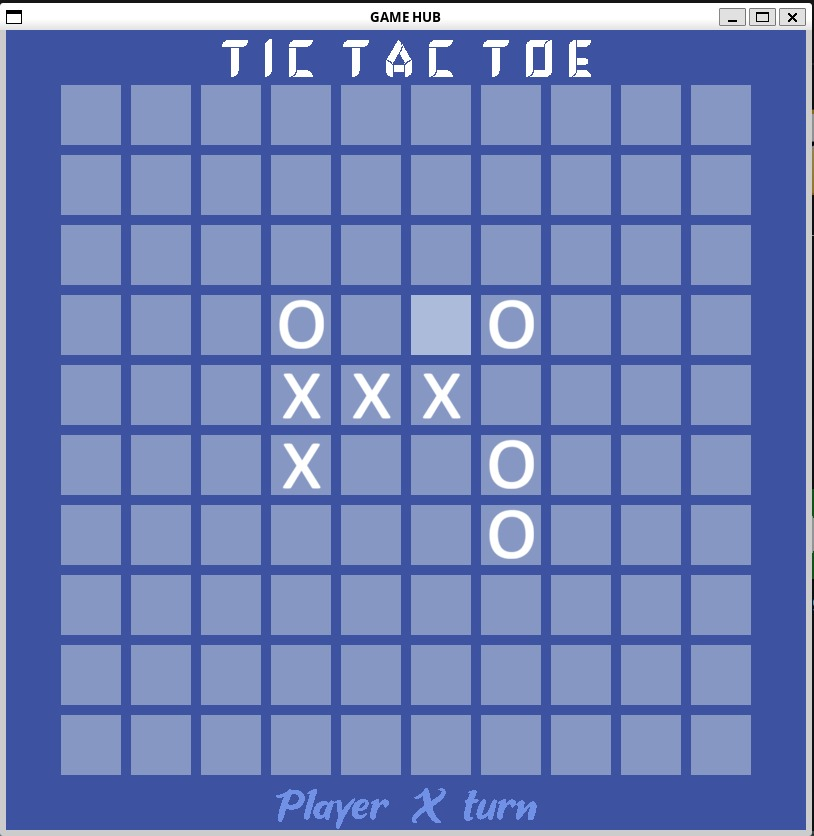
\includegraphics[width=0.5\textwidth]{tictactoe.png}
    \caption{Tic-Tac-Toe}
    \label{fig:menu}
    \end{figure}
    
    \textbf{Connect 4}\\
    Connect 4 is played on a 7×7 grid where the goal is to align four consecutive discs. The board is again stored using a NumPy array, and each column has an associated \texttt{level} value that tracks how many discs are already placed in that column.
    
    When a player selects a column, the disc is assigned to the lowest available position using:
    \begin{center}
    \texttt{row = 6 - level[col]}
    \end{center}
    This simulates gravity, ensuring that pieces stack correctly from bottom to top.
    
    After placing a disc, the turn switches to the other player, and the win-checking process begins.
    
    The win detection logic closely mirrors the Tic-Tac-Toe approach but uses sequences of length 4 instead of 5. Horizontal checks are performed by slicing the board into overlapping groups of four columns and applying \texttt{all(axis=1)}. Vertical checks use similar slicing across rows.
    
    For diagonal detection, multiple 4×4 submatrices are extracted from the board. These submatrices are shifted step-by-step and combined using logical AND operations. If any position remains True after combining, it indicates four aligned discs diagonally.
    
    This method ensures that all possible diagonal combinations are checked efficiently without explicitly looping over each diagonal. As soon as any valid sequence is found, the game state is updated to indicate completion.
    
              \begin{figure}[h]
    \centering
    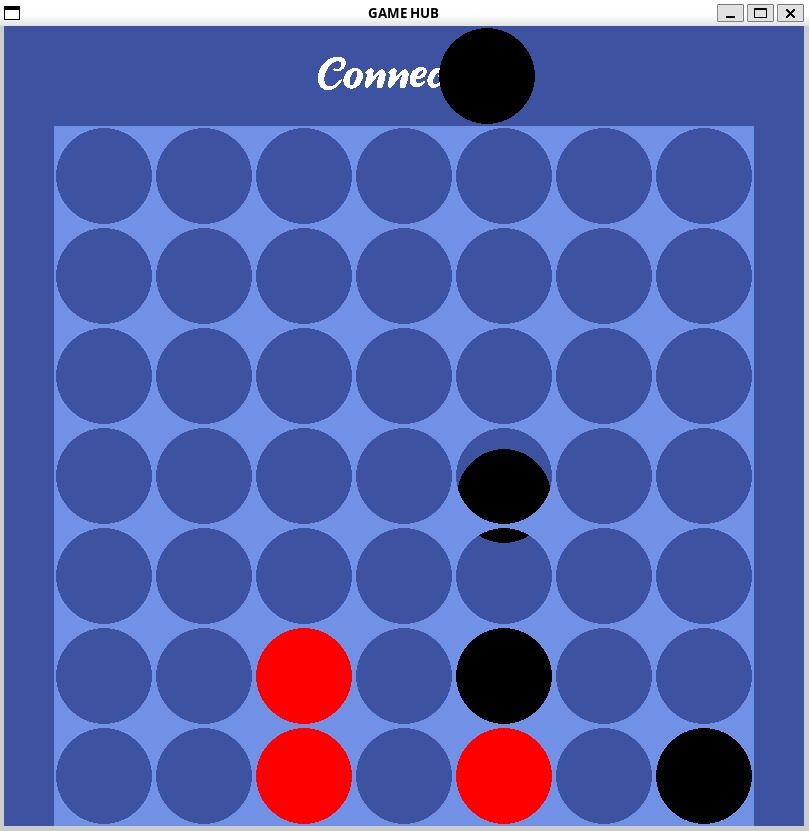
\includegraphics[width=0.5\textwidth]{connect4.png}
    \caption{Connect4}
    \label{fig:menu}
    \end{figure}
    
    \textbf{Othello (Reversi)}\\
    Othello is played on an 8×8 grid, where the main challenge lies not in placement, but in flipping the opponent’s discs. The board is represented using a NumPy array where \texttt{0} denotes Black, \texttt{1} denotes White, and \texttt{None} indicates an empty cell.
    
    The core logic revolves around validating moves and flipping discs correctly. A move is only valid if placing a disc captures at least one opponent disc. This is handled by the \texttt{check\_and\_flip} function, which checks all four directions: horizontal, vertical, and two diagonals.
    
    At the heart of this process is the \texttt{checkline} function. Given a one-dimensional slice of the board (row, column, or diagonal), it examines both forward and backward directions from the chosen position. It searches for a sequence where opponent discs are followed by a disc of the current player. If such a pattern is found, all intermediate discs are flipped.
    
    For horizontal and vertical checks, rows and columns are directly extracted from the array. For diagonal checks, NumPy’s \texttt{diagonal()} function is used. In the case of the anti-diagonal, the board is flipped using \texttt{fliplr()} before extracting the diagonal.
    
    If any direction results in a successful flip, the move is considered valid, and the board is updated in-place.
    
    The game also includes a recursive function \texttt{has\_any\_valid\_move}, which scans all empty cells to determine whether a player has at least one valid move. If a player cannot move, the turn is passed back. If neither player has a valid move, the game ends.
    
    Finally, the winner is determined by counting the number of discs using:
    \begin{center}
    \texttt{np.sum(used == 0)} and \texttt{np.sum(used == 1)}
    \end{center}
    
    This implementation focuses heavily on array manipulation and avoids unnecessary loops, making the logic both efficient and clean.

          \begin{figure}[h]
    \centering
    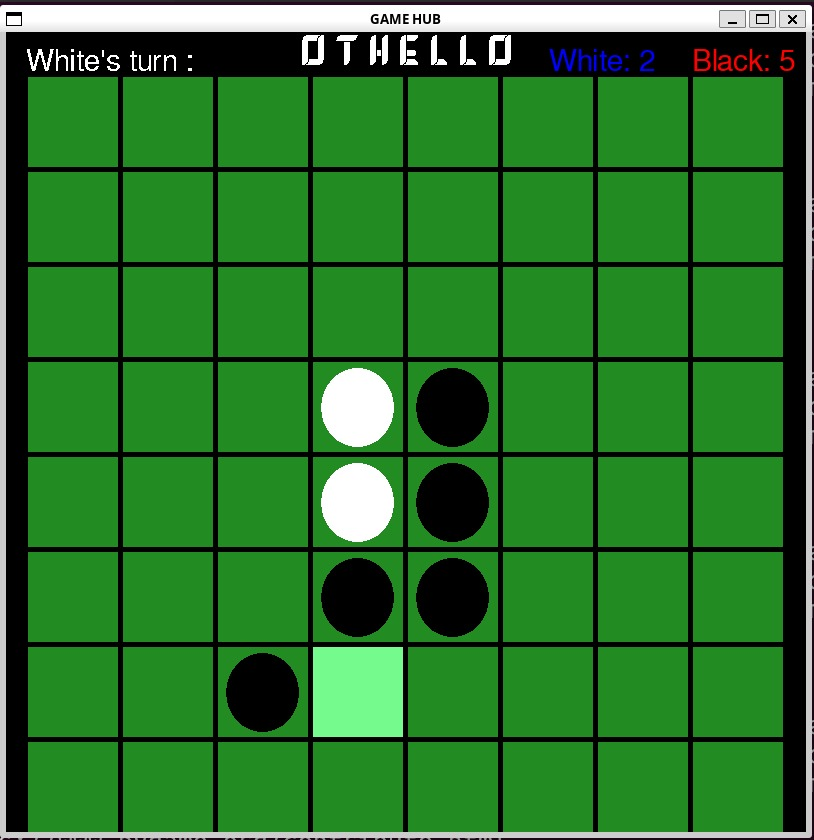
\includegraphics[width=0.5\textwidth]{othello.png}
    \caption{Othello}
    \label{fig:menu}
    \end{figure}
    \newpage
    \section{Leaderboard and Analytics}
    After each match, the Python engine appends the result to \texttt{history.csv}. The \texttt{leaderboard.sh} script then processes this data using \texttt{awk} and \texttt{sort} to rank players. At the same time, \texttt{matplot.py} creates visual charts of the players' performance history.
    \begin{figure}[h]
        \centering
        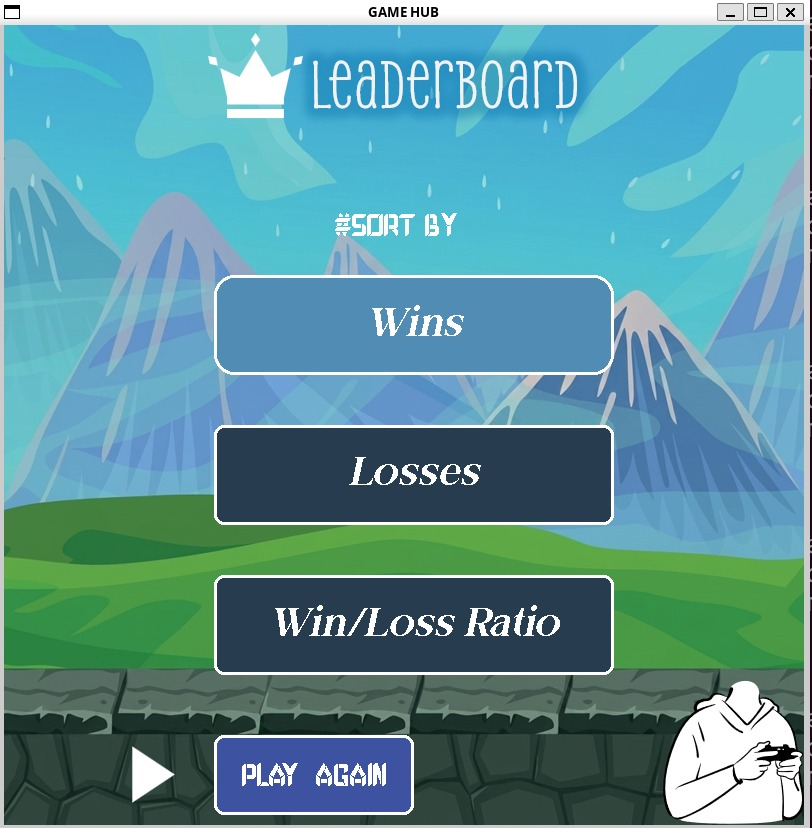
\includegraphics[width=0.5\textwidth]{leaderboard.png}
        \caption{Post-game Leaderboard and Analytics Dashboard}
        \label{fig:leaderboard}
    \end{figure}

    \section{Hurdles and Solutions}
    \begin{itemize}
        \item \textbf{Hurdle:} Passing data smoothly between Bash scripts and Python scripts. \\
        \textbf{Solution:} Used \texttt{subprocess} and shared CSV files to communicate between languages.
        \item \textbf{Hurdle:} Checking win conditions on large grids without slow loops. \\ 
        \textbf{Solution:} Leveraged NumPy functions like \texttt{diagonal()}, \texttt{all()}, and \texttt{fliplr()} for instant matrix checks.
    \end{itemize}

    \section{The "10-Hour" Plan}
    If we had 10 additional hours, we would implement a Single Player mode featuring an machine opponent so users can play even when a second player is not available.
    definitely we would improve our project .

    \begin{thebibliography}{}
        \bibitem{python} Python inheritance: \url{https://docs.python.org/3/tutorial/classes.html}
        \bibitem{pygame} Pygame CE Documentation: \url{https://inventwithpython.com/pygame/}
    \end{thebibliography}

\end{document}